\documentclass[tikz]{standalone}
\usepackage{pgfplots}
\pgfplotsset{compat=1.15}
\usepackage{mathrsfs}
\usetikzlibrary{arrows,calc}
\usepackage{tkz-euclide}
\pagestyle{empty}

\definecolor{AngleClr}{rgb}{0,0.39215686274509803,0}
\definecolor{ShapeClr}{rgb}{0.6,0.2,0}

\begin{document}

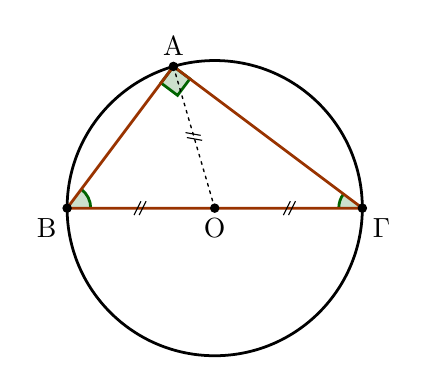
\begin{tikzpicture}[scale=.75]
\tkzSetUpLine[line width=1pt,color=black]
\tkzSetUpPoint[fill=black]

\tkzDefPoints{0/0/B,1.8/2.4/A,5/0/C}

\tkzDefCircle[circum](A,B,C) \tkzGetPoint{O}
\tkzDrawCircle[line width=1.0pt, color=black](O,A)

\tkzDefMidPoint(A,B) \tkzGetPoint{M1}
\tkzDefMidPoint(B,C) \tkzGetPoint{M2}
\tkzDefMidPoint(A,C) \tkzGetPoint{M3}

\tkzFillPolygon[fill=white](A,B,C)

\tkzMarkRightAngle[line width=1pt, size=.35,color=AngleClr,fill=AngleClr,fill opacity=0.2](B,A,C)
\tkzFillAngles[fill=AngleClr,size=.4,fill opacity=0.2](C,B,A A,C,B)
\tkzMarkAngles[line width=1pt,size=.4,color=AngleClr](C,B,A A,C,B)

\tkzDrawSegments[line width=0.5pt,color=black,dashed,dash pattern=on 1pt off 1.75pt](O,A O,B O,C)


\tkzDrawPolygon[color=ShapeClr](A,B,C)
\tkzDrawPoints[size=3](A,B,C,O)
\tkzLabelPoint[above](A){$\rm A$}
\tkzLabelPoint[below left](B){$\rm B$}
\tkzLabelPoint[below right](C){$\rm \Gamma$}
\tkzLabelPoint[below](O){$\rm O$}

\tkzMarkSegments[mark=s||,size=2.5](O,A O,B O,C)

\end{tikzpicture}

\end{document}